\section{组合图}
\label{sec:composite-plots}

前面介绍的绘图命令五花八门,但无论是 \texttt{plot}、\texttt{plot1} 或是
\texttt{plot2},同一个窗口内绘制的所有波形总是共用同一个X轴。实际绘图时,
经常需要在一张图中绘制多个不同X轴的图,即组合图。

SAC提供了绘制组合图的功能,这其中牵涉到一些新的概念,其中之一是
\texttt{frame}。一般而言,在执行绘图命令时会首先对整个窗口进行擦除。
比如,先执行 \texttt{plot} 命令,窗口中会显示出相应的波形,然后执行
\texttt{plot1} 命令,首先会将窗口中的已有图像全部擦除,再绘制相应波形。

在frame中,每次执行绘图命令时,不会擦除窗口中的已有图像,从而实现了将
多个命令的绘图效果同时显示在一个窗口中。使用 \nameref{cmd:beginframe}
打开frame时,首先会擦除整个窗口,进入``组合图模式'';当组合图绘制完成时,
需要使用 \nameref{cmd:endframe} 命令关闭frame。

除了frame之外,在绘制组合图时还需要了解与窗口有关的几个概念,如图
\ref{fig:window-viewspace-viewport}:
\begin{itemize}
\item window:图形窗口。对于xwindows图形设备,window如图 \ref{fig:plot}
    所示,其默认长宽比为11.0/8.5=1.294;对于sgf图形设备,可以认为window
    的大小即为A4纸张的大小。
\item viewspace:window内可以用于绘图的部分;
\item viewport:执行单个绘图命令时,图像的显示区域;
\end{itemize}

\begin{figure}[H]
\centering
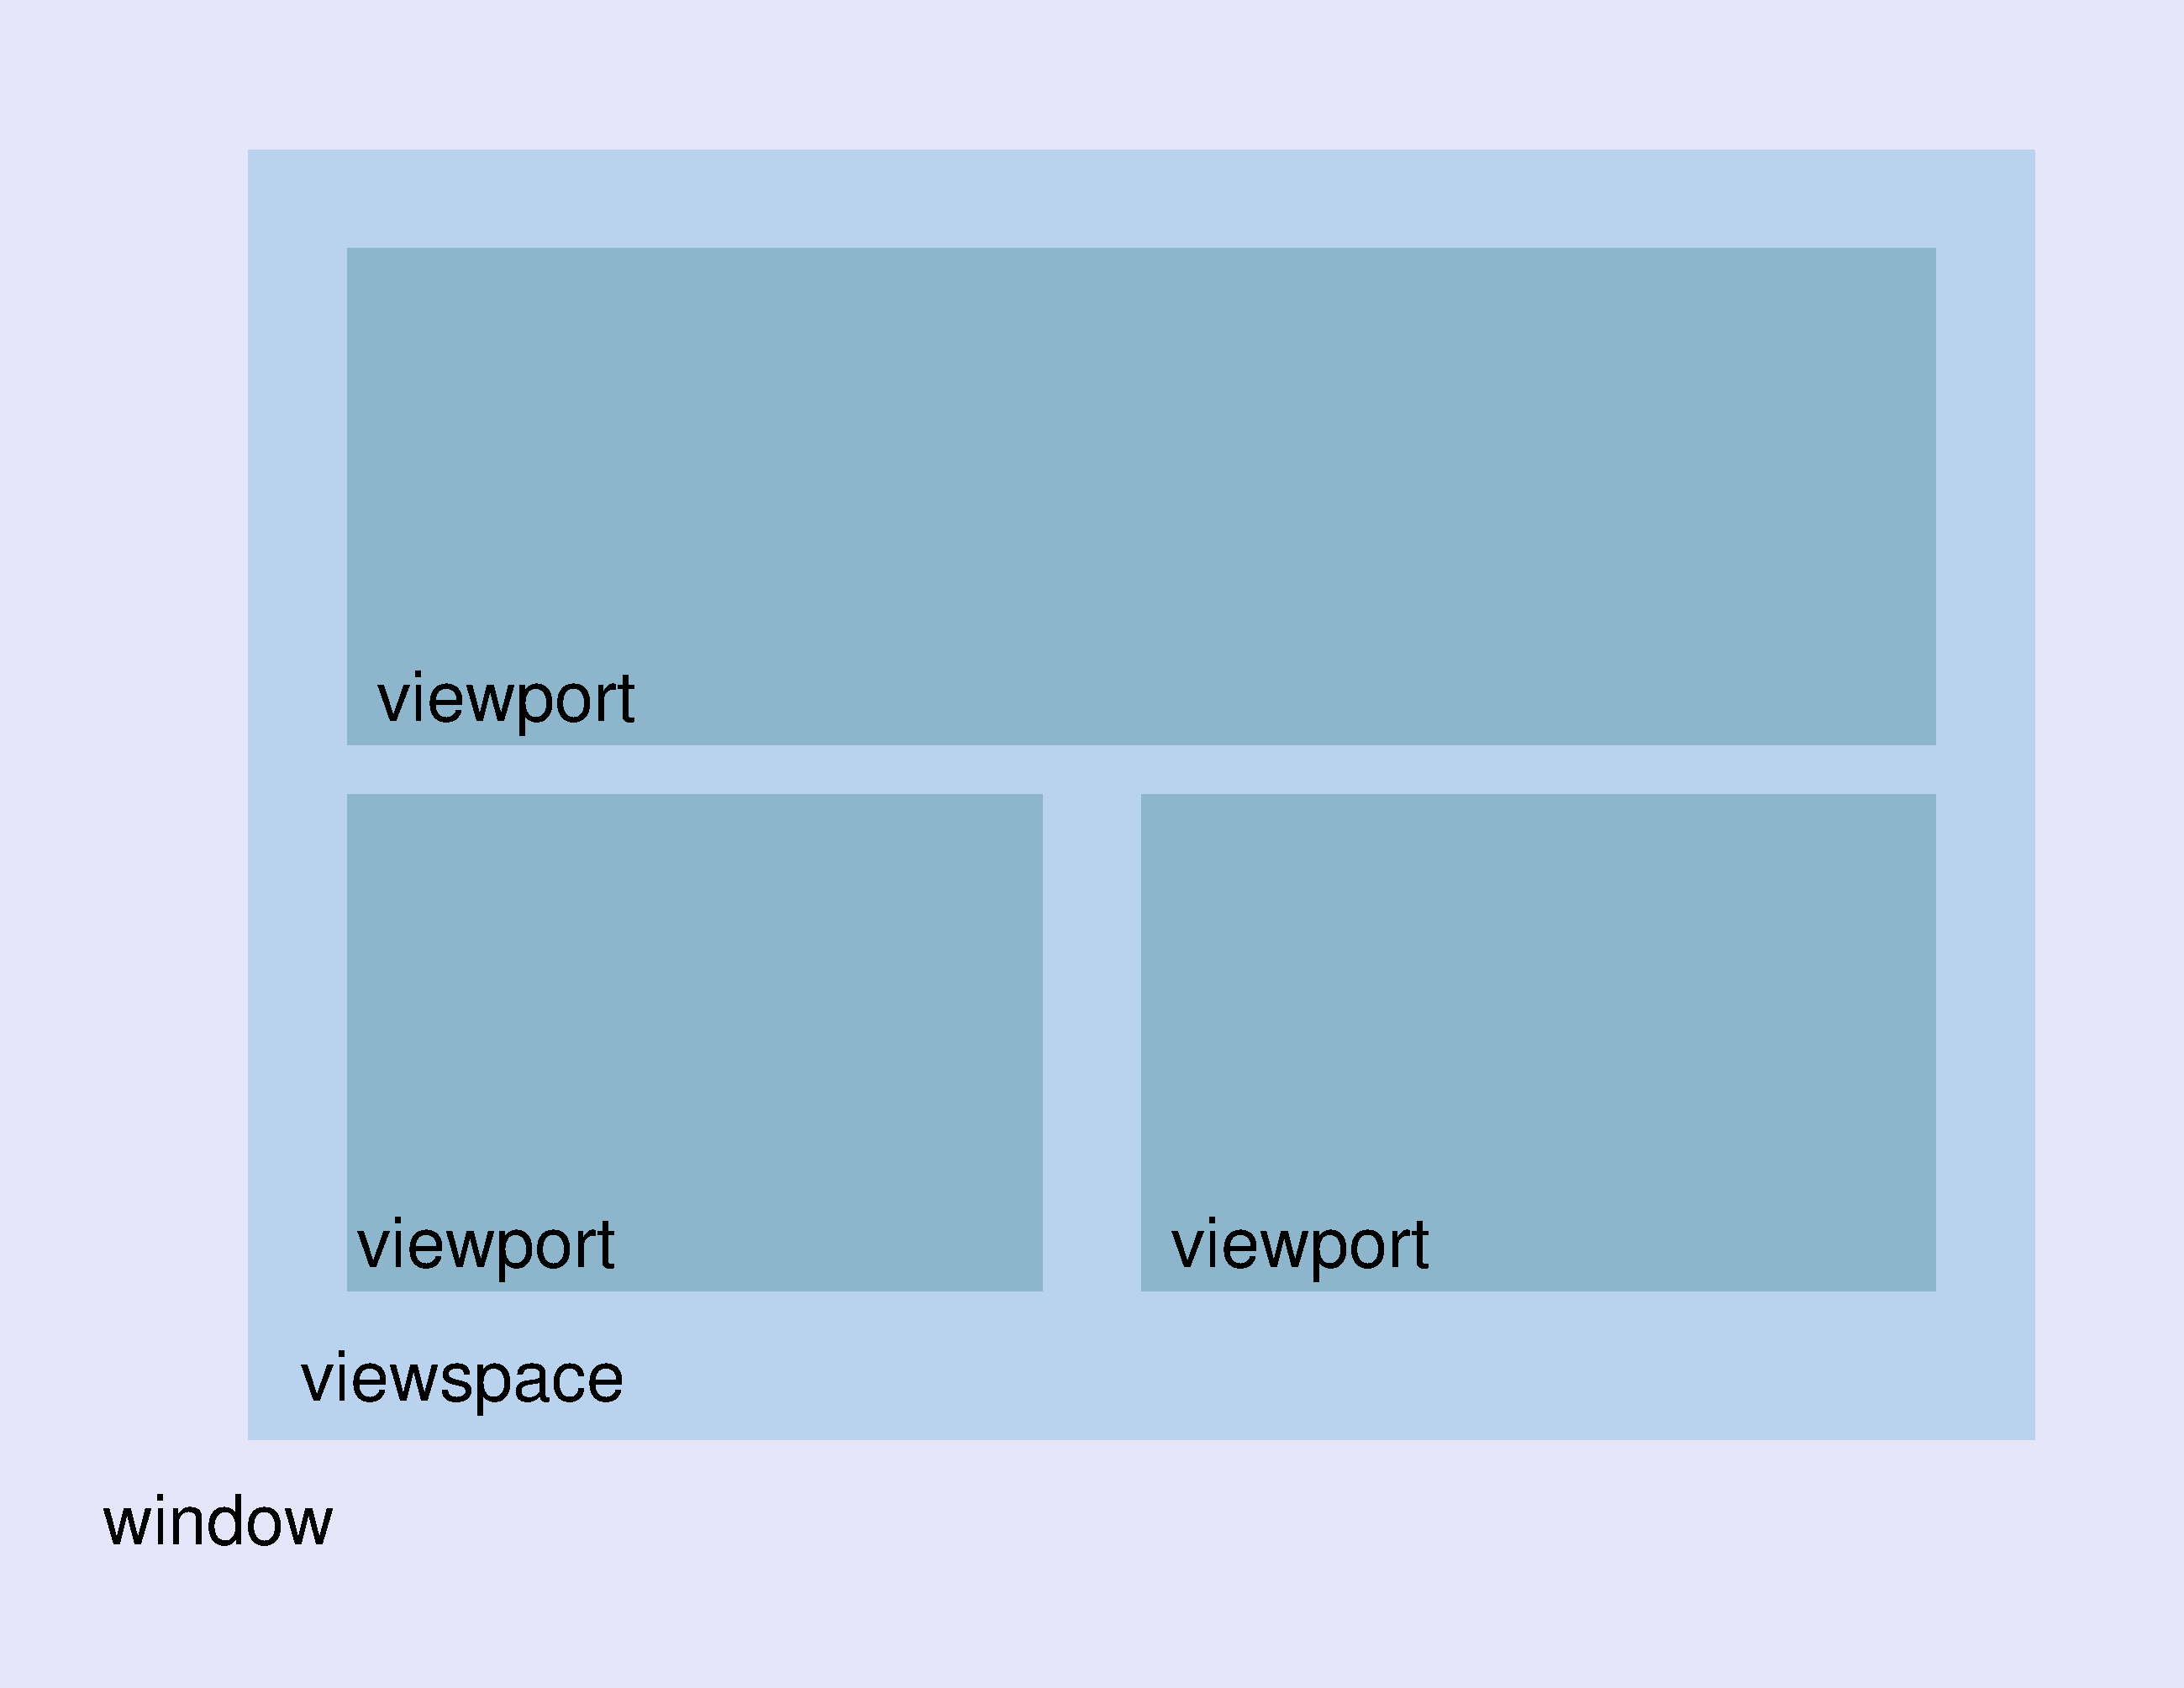
\includegraphics[width=0.8\textwidth]{viewspace-viewport}
\caption{window、viewspace和viewport}
\label{fig:window-viewspace-viewport}
\end{figure}

图 \ref{fig:window-viewspace-viewport} 中给出了window、viewspace、
viewport的相互关系。可以使用 \nameref{cmd:window} 命令设定窗口相对于
整个屏幕的位置以及X、Y方向的范围;\nameref{cmd:vspace} 用于设定整个
绘图区的比例;\nameref{cmd:xvport} 和 \nameref{cmd:yvport} 则分别定义
了单个绘图命令所能使用的X、Y方向的范围。

一个典型的组合图的绘制如下所示:
\begin{SACCode}
SAC> fg seis                        // 生成数据
SAC> beginframe                     // 打开frame,开始绘制组合图
SAC> xvport 0.1 0.9                 // 设定第一个绘图命令的viewport
SAC> yvport 0.7 0.9
SAC> title 'Seismic Trace'          // 设定标题
SAC> fileid off                     // 不显示文件id
SAC> qdp off
SAC> p
SAC> fft wmean                      // FFT
SAC> xvport .1 .45                  // 设定第二个绘图命令的viewport
SAC> yvport .15 .55
SAC> title 'Amplitude Response (linlog)'
SAC> ylim 1e-5 1                    // Y轴范围
SAC> psp am linlog                  // 绘制振幅谱
SAC> xvport .55 .9                  // 设定第三个绘图命令的viewport
SAC> title 'Amplitude Response (loglog)'
SAC> xlim 1 60
SAC> psp am loglog                  // 绘制振幅谱
SAC> endframe                       // 关闭frame
\end{SACCode}

\begin{figure}[H]
\centering
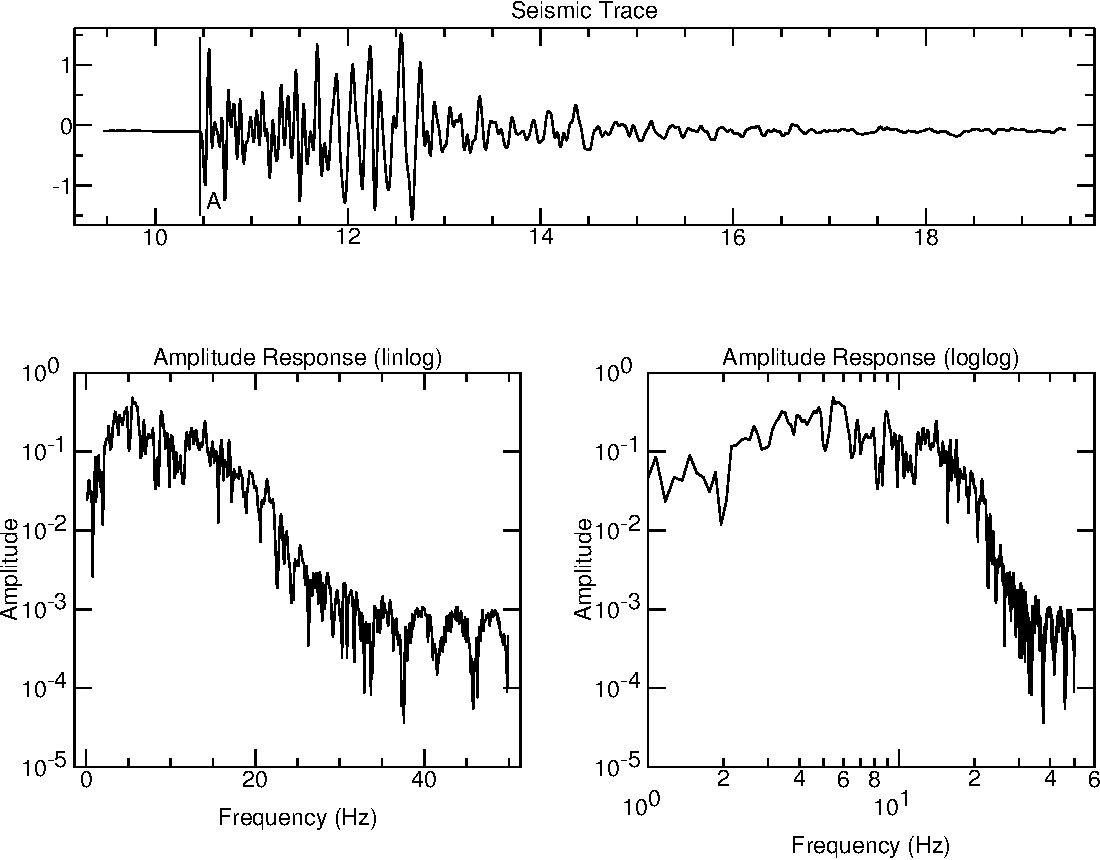
\includegraphics[width=0.9\textwidth]{composite-plot}
\caption{绘制组合图}
\label{fig:composite-plot}
\end{figure}
